\section{Программная реализация}

После изучения алгоритма Тарского была начата работа по реализации этого алгоритма, но не для произвольных формул, а для формул без параметров.

\begin{definition}
    Формула $\mathcal{A}$ называется \textbf{формулой без параметров}, если для любой ее подформулы вида $(Qx)\mathcal{B}$, формула $\mathcal{B}$ свободна от вхождений кванторов и от переменных, возможно, за исключением переменной $x$.
\end{definition}

Для этого были выбраны язык C\#, платформа .NET Core 3.1 и спецификация .NET Standard 2.1 \cite{TroelsonNet}. Такой выбор обусловлен рядом причин:
\begin{itemize}
    \item Язык C\#~--- это объектно-ориентированный язык программирования, а данная парадигма программирования позволяет абстрактно описывать объекты, в том числе и математические объекты; 
    \item .NET Core и .NET Standard~--- это современные, развивающиеся и востребованные кроссплатформенные технологии с открытым исходным кодом;
    \item Личные предпочтения автора.
\end{itemize}
Для поэтапного создания программы, были сформулированы и решены следующие задачи:
\begin{itemize}
    \item Разработать библиотеку классов для объектов языка элементарной алгебры: символы алфавита, термы, формулы;
    \item Реализовать ввод логических формул, то есть решить задачу лексического анализа, решить задачу синтаксического анализа;
    \item Разработать библиотеку классов для рациональных чисел и многочленов от одной вещественной переменной с рациональными коэффициентами;
    \item Реализовать алгоритм Тарского для формул от одной переменной;
    \item Реализовать алгоритм элиминации кванторов (утверждение \ref{algB}) для формул без параметров;
    \item Провести тестирование модулей, интеграционное и end-to-end тестирования;
    \item Собрать все библиотеки и модули в единый программный комплекс.
\end{itemize}
Написание программы осуществлялось в среде разработки Microsoft Visual Studio 2019 Community с установленным дополнением ReSharper. Обе программы доступны по специальным студенческим лицензиям для использования в некоммерческих целях.

\subsection{Представление формул}

Необходимо было начать с того, что создать абстракции для всех объектов языка элементарной алгебры: символы алфавита, термы, формулы. Для этого была написана библиотека классов IOLib, в которой определены следующие пространства имён:
\begin{itemize}
    \item в IOLib.Exceptions расположены классы для ошибок, исключительных ситуаций, возникающих при разборе входной строки;
    \item в IOLib.Input~--- классы и интерфейсы, определяющие токенизацию, парсинг и трансляцию;
    \item в IOLib.Language~--- определены классы, моделирующие объекты языка, а именно символы, термы  формулы;
    \item в IOLib.Output~--- интерфейс и классы для обратного преобразования формулы в строку в LaTeX-like формате.
\end{itemize}

\subsubsection{Класс Symbol}

Начнём с класса Symbol. Он предоставляет представление в виде строки (string), реализует интерфейс IEquatable<Symbol>, чтобы иметь возможность сравнивать символы. Сравнение происходит путём сравнения строковых представлений символов.

Далее следует рассмотреть статический класс Alphabet, который предоставляет множество полей, каждое из котоых имеет тип Symbol и моделирует один из символов входного языка. Также класс предоставляет несколько методов для работы с буквами и цифрами, а именно получение соответствующего символа по объекту типа char, проверка является ли данный объект типа Symbol буквой или цифрой.

Было принято решение отказаться от архитектуры, используемой в предыдущих работах, когда под каждый символ создавался класс. Это приводило к тому, что код содержал много однотипных сущностей без методов, полей и свойств. Новая архитектура решает задачи, которые обычно решают с помощью паттерна одиночка, который в свою очередь был не применим в предыдущем подходе из-за наследования.

\subsubsection{Класс Term}

Прежде чем перейти к описанию формул, необходимо описать класс для термов языка элементарной алгебры. При определении терма выделяется три случая: константа, переменная, функция от термов. Поэтому абстрактный класс Term является базовым для трех классов. Чтобы для формул находить список переменных, входящих в терм, объявлено абстрактное свойство ObjectVariables, которое очевидным образом реализуют наследники.

Первый и второй классы оборачивают константы и переменные, а третий хранит функцию и массив аргументов, то есть другие термы.

\subsubsection{Класс Formula}

И наконец, объект, для которого были написаны все ранее перечисленные классы~-- формула языка элементарной алгебры. Вновь, исходя из определения формулы получается такая иерархия классов: во главе абстрактный класс Formula и три класса-наследника.

Класс PredicateFormula описывает формулы вида $p\left(t_1, ... , t_n\right)$, где $p$~-- $n$-местный предикат, а $t_i$~--- терм. Класс PropositionalConnectiveFormula, в котором объявлены поля для пропозициональной связки и аргументов, описывает формулы вида $\mathcal{A} * \mathcal{B}$, где $* \in \left\{\&, \lor, \to\right\}$, или вида $\neg \mathcal{A}$. И для формул вида $(Qx)(\mathcal{A})$ реализован класс QuantifierFormula.

В результате, описаны все объекты языка элементарной алгебры. При этом данная система допускает расширение, например, можно добавлять логические связки, функции или вводить новые предикаты.

\subsection{Система ввода}

Далее необходимо реализовать методы, преобразующие введенную пользователем строку в формулу, то есть в экземпляр класса Formula, или, сообщают о том, что данная строка не является формулой. Аналогичная задача, но для формул исчисления высказываний, была успешно решена в предыдущей работе \cite{Gibadulin1}. Однако и в этом аспекте было решено изменить подход к решению задачи. Отказаться от алгоритма Дейкстры и ОПЗ в пользу классического метода решения задачи синтаксического анализа~--- разбор формулы по грамматике нисходящим разбором.

Задачу лексического анализа можно решить с помощью конечных автоматов. Интерфейс ITokenizer определяет функцию, которая будет решать эту задачу, то есть по строке на входы выдавать последовательность символов на выходе.

Была задана входная грамматика, каждый символ закодирован строкой также, как это делается в системе LaTeX и получен набор лексем или ещё их называют токенами. Далее был придуман и реализован следующий алгоритм: по токенам строится префиксное дерево, затем это дерево преобразуется в автомат Мили, то есть в автомат с выходом.

Синтаксический анализ осуществляется алгоритмом нисходящего разбора. В общем случае этот алгоритм является экспоненциальным, однако для данной грамматики можно показать, что алгоритмы понадобиться шагов не более чем константа умноженная на квадрат от количества символ в строке.

\subsection{Реализация алгоритма Тарского}

Переходим непосредственно к реализации алгоритма построения бескванторной формулы, а точнее к рассмотрению библиотеки SimpleTarskiAlgorithmLib.

Первым делом рассмотрим перечисление Sign, так как именно знаки чисел и многочленов являются важной и при этом самой простой частью алгоритма. В этом перечислении определены следующие значения:
\begin{itemize}
    \item NotNumber~--- объект не имеет знака;
    \item LessZero~--- меньше нуля;
    \item MoreZero~--- больше нуля;
    \item Zero~--- нуль;
    \item NotMoreZero~--- не больше нуля;
    \item NotLessZero~--- не меньше нуля;
    \item NotZero~--- не нуль; 
    \item Undefined~--- знак может быть любым.
\end{itemize}

Так как рассматриваются многочлены с коэффициентами из $\mathbb{Q}$, необходимо реализовать структуру для рациональных чисел. Для этого достаточно в качестве целых чисел взять структуру BigInteger и вспомнить как определяются рациональные числа и операции над ними в алгебре. Поэтому для этой структуры определены поля для числителя и знаменателя, а также поле для знака числа. Естественным образом реализованы арифметические операции сложение, вычитание, умножение, деление и возведение в натуральную степень.

Для реализации класса для многочленов вновь необходимо вспомнить как они определяются в алгебре и реализовать эти определения в виде программы. Поэтому в классе Polynomial определен массив из рациональных чисел, переменная типа VariableName и поля для знака многочлена. Как в алгебре старший коэффициент многочлена отличен от нуля, так и элемент массива с наибольшим индексом не должен быть равным нулю. Для многочленов определены операции сложения, вычитания, умножения, деление с остатком, формальное дифференцирование и возведение в натуральную степень.

Переходим к задаче насыщения системы многочленов. Для её решения создан статический класс SimpleSaturator, а точнее его метод Saturate. На вход ему поступает последовательность многочленов. Затем он из них выбирает все ненулевые, вычисляет производную их произведения и помещает выбранные многочлены и производную в очередь. Далее пока очередь не пуста происходит следующее:
\begin{itemize}
    \item Извлекаем из очереди первый многочлен $P$. Если он уже добавлен в результирующее множество, то есть в HashSet<Polynomial>, то переходим к следующей итерации цикла;
    \item Добавляем в очередь производную этого многочлена;
    \item Для каждого многочлена $Q$ из результирующего множества добавляем его остаток от деления на $P$, если $deg(Q) \geq deg(P)$, и остаток от деления $P$ на $Q$, если $deg(P) \geq deg(Q)$.
\end{itemize} 

После этапа насыщения системы следует этап построения таблицы Тарского, поэтому необходимо реализовать структуру данных соответствующую свойствам таблицы. Во-первых, довольно часто будут добавляться столбцы, поэтому предлагается рассматривать таблицы как связный список столбцов, что позволяет наиболее эффективно добавлять новые столбцы. Во-вторых, строки добавляются только в конец таблицы, поэтому столбцы представляют собой список знаков~--- List<Sign>, так как добавление в конец списка и обращение к элементу списка происходят достаточно быстро.

Рассмотрим последнюю библиотеку~--- SimpleTarskiAlgorithmRunner. Именно класс SimpleTarskiAlgorithm, расположенный в этой библиотеке, связывает формулы и алгоритм Тарского. QuantifiersElimination~--- единственный публичный метод этого класса. Он реализует алгоритм $B$, описанный в утверждении \ref{algB}, а алгоритм $A$, то есть алгоритм Тарского для формулы вида $(Qx)\Phi(x)$, реализован в виде метода TarskiEliminate.

На этом заканчивается описание программы. Исходный код проекта размещен в виде репозитория на GitHub, ссылку на который можно найти в приложении А. Еще в репозитории можно найти проекты с юнит-тестами, так как весь код отлаживался, а наиболее сложные его части тестировались.

\subsection{Демонстрация работы}

Чтобы продемонстрировать работу программы было создано простое консольное приложение. Пользователю предлагается ввести формулу. После того как пользователь ввел формулу ему выводится сообщение о том, в какой файл записан результат работы программы. Далее (рис. \ref{fig:примеры}) приведено несколько примеров содержания таких выходных файлов.

Для того, чтобы реализовать алгоритм Тарского для формул общего вида, необходимо, во-первых, реализовать многочлены с параметрами, во-вторых, насыщение системы. Если с многочленами сложностей не возникает (в проекте уже реализован соответствующий класс), то насыщение системы таких многочленов оказалось нетривиальной задачей, так как требует разбора случаев знака коэффициентов. При этом построение таблицы и остальные части, за редким исключением, не отличаются от того, что уже было реализовано. Поэтому можно сказать, что в данной работе реализован базовый, но наиболее важный и трудоёмкий случай.


\begin{figure}[ht]
    \begin{minipage}[ht]{0.349\linewidth}
        \center{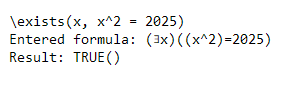
\includegraphics[width=0.99\linewidth]{пример1.PNG} \\ а)}
    \end{minipage}
    \hfill
    \begin{minipage}[ht]{0.65\linewidth}
        \center{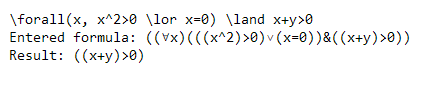
\includegraphics[width=0.99\linewidth]{пример2.PNG} \\ б)}
    \end{minipage}
    \\
    \begin{center}
        \begin{minipage}[ht]{0.8\linewidth}
            \center{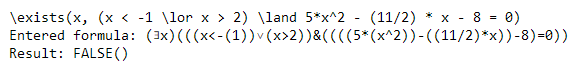
\includegraphics[width=0.99\linewidth]{пример3.PNG} \\ в)}
        \end{minipage} 
    \end{center}
    \caption{Примеры выходных данных.}  
    \label{fig:примеры}
\end{figure}